% !TEX root = morphkasten.tex

\section{Microcontroller}


%##############
\subsection{Freedom-Board}
\begin{figure}[h]
	\centering
	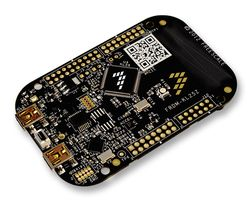
\includegraphics[width=0.5\textwidth]{fig/freedomboard.png}
	\caption{Freedomboard KL25 von Freescale (Quelle:http://ch.farnell.com/)}
	%http://ch.farnell.com/productimages/standard/de_DE/freescalesemiconductor-frdm-kl25z-40.jpg
\end{figure}


\begin{table}[h]
\begin{tabular}{p{0.5\textwidth} | p{0.5\textwidth}}


 \textbf{Vorteile} & \textbf{Nachteile} \\ \hline
	 
\begin{itemize}
\item Im Preisrahmen, ein Board gibt es ab 20Fr.-
\item Wurde an der Hochschule bereits eingesetzt(mögliche Ansprechpersonen)
\item Vereinfachte Programmierung mit Processor Expert
\item Kann zu Testzwecken ausgeliehen werden
\end{itemize}

 &
 
\begin{itemize}
\item Besitzt ein Betriebssystem $\Rightarrow$ weniger Hardware nahe
\item Keine zusätzlichen Module (weitere Hardware muss angebunden werden)
\end{itemize}

\end{tabular}
\end{table}

\begin{table}[h]
\begin{tabular}{p{0.5\textwidth}p{0.5\textwidth}}


 \textbf{Risiken} & \\ \hline
	 
\begin{itemize}
\item Die Anbindung möglicher Sensoren/Aktoren ist schwieriger als erwartet
\item Die Kommunikation zum Bordcomputer ist nicht ausreichend (unwahrscheinlich)
\end{itemize}
&
\begin{itemize}
\item Die Anzahl AD-Eingänge reicht nicht aus (unwahrscheinlich)
\end{itemize}

 
\end{tabular}
\end{table}

\pagebreak


%##############
\subsection{Tinkerforge}
\begin{figure}[h]
	\centering
	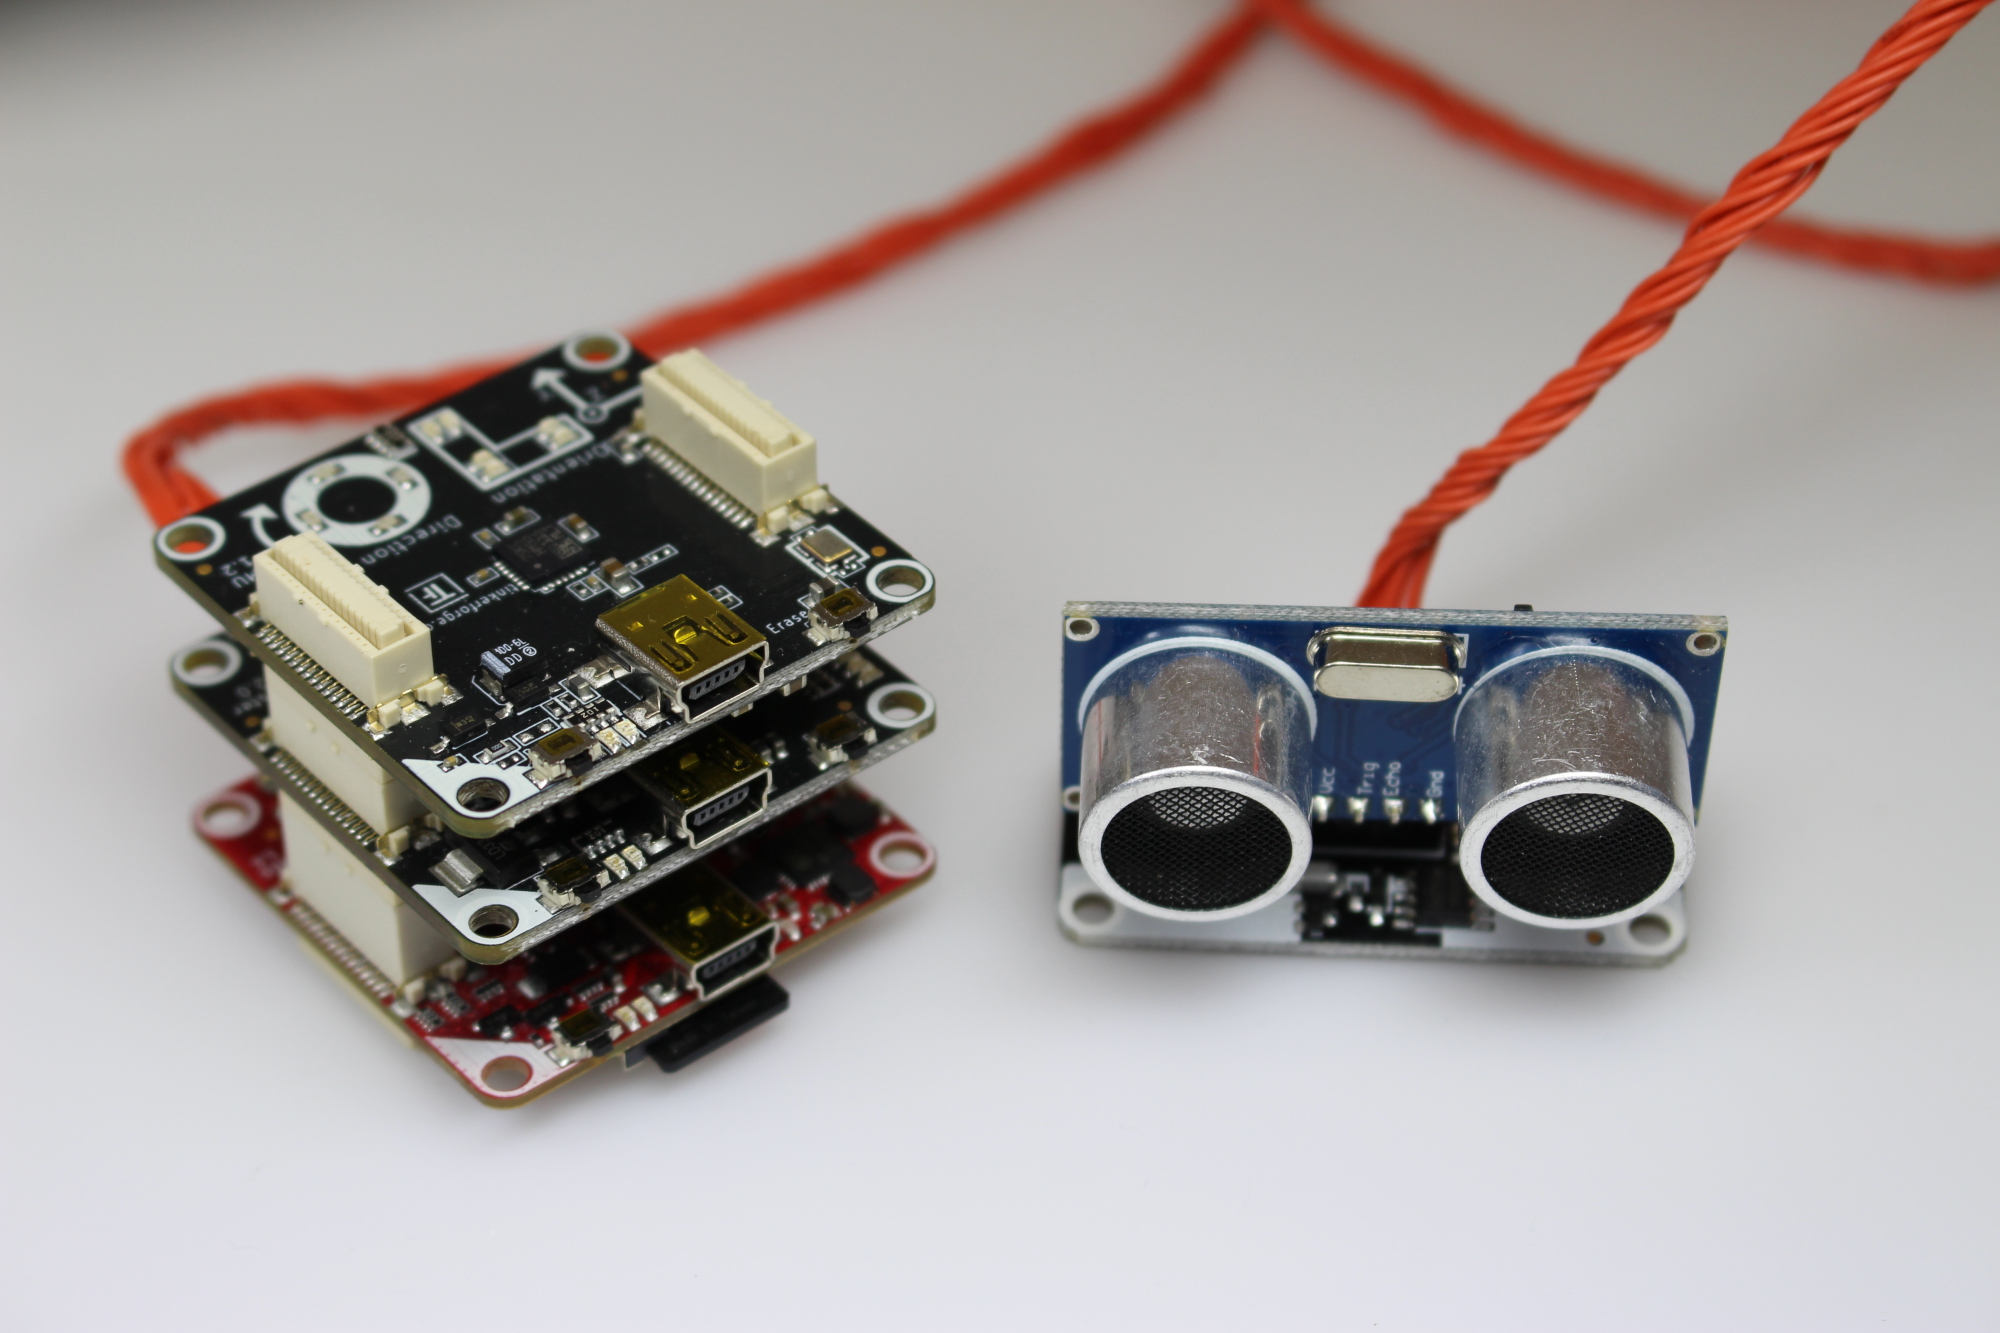
\includegraphics[width=0.5\textwidth]{fig/Tinkerforge.png}
	\caption{Beispielhaftes Tinkerforge System (Bricks mit Ultraschallmodul) (Quelle: http://www.heise.de)}
	%http://www.heise.de/imgs/18/1/3/9/9/7/1/4/IMG_0866-6a15d221db4848a1.jpeg
\end{figure}

\begin{table}[h]
\begin{tabular}{p{0.5\textwidth} | p{0.5\textwidth}}


\textbf{Vorteile} & \textbf{Nachteile} \\ \hline
	 
\begin{itemize}
\item Einfache und modulare Schnittstelle zum Boardcomputer
\item Einfach erweiterbar mit zusätzlichen Modulen (z.B Sensoren)
\item Viele benötigte Module Vorhanden: Schrittmotoren, Distanzsensoren, Liniensensoren und Farbsensoren
\end{itemize}
 &
\begin{itemize}
\item Grosser Aufwand für eigene Module (Abhängigkeit zu Tinkerforge)
\item Debugging könnte Probleme bereiten (Linuxberiebsystem) 
\end{itemize}
\end{tabular}
\end{table}


\begin{table}[h]
\begin{tabular}{p{0.5\textwidth}p{0.5\textwidth}}


\textbf{Risiken} & \\ \hline
	 
\begin{itemize}
\item Es sind nicht alle benötigten Module vorhanden oder erfüllen die Anforderungen => eventuell aufwändige Hardwareanbindung nötig
\item Die Rechenperformance reicht nicht (unwahrscheinlich)
\end{itemize}
&
\begin{itemize}
\item Teure Hauptplatine, ein Defekt könnte das Budget belasten.
\item Lieferung aus Deutschland, eventuelle lange Lieferzeit (wichtig bei Defekt)
\end{itemize}

 
\end{tabular}
\end{table}

\pagebreak